\begin{frame}
    \begin{center}
        \Huge ¡Bienvenidos!
    \end{center}
\end{frame}

\begin{frame}{Matrícula inicial}
    \begin{figure}
        \centering
        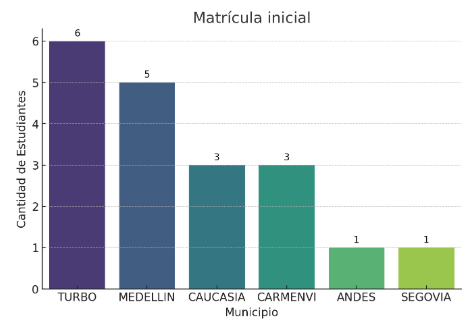
\includegraphics[width=0.5\linewidth]{figures/matricula-inicial.png}
    \end{figure}
\end{frame}

\begin{frame}{Generalidades}
    \begin{itemize}
        \item Horario de clases: martes y jueves 20:00 $-$ 22:00
        \item Clases en Zoom
        
        \begin{itemize}
            \item Enlace: {\color{blue}\url{udearroba.zoom.us/j/93686452220}}
            \item Meeting ID: 936 8645 2220
        \end{itemize} 
        \item Las sesiones se dividirán en:
        \begin{itemize}
            \item Teoría: aproximadamente una hora
            \item Práctica: aproximadamente 40 minutos
        \end{itemize}
        \item Horario de asesorías: martes 14:00 $-$ 15:00
        \begin{itemize}
            \item Virtual: {\color{blue}\url{meet.google.com/dgr-qdvk-qpr}}
            \item Presencial: sede Medellín Ciudad Universitaria, aula 6-120.
        \end{itemize}
        
    \end{itemize}
\end{frame}

\begin{frame}{Generalidades}
    \begin{itemize}
        \item Textos guía:
        \begin{itemize}
            \item Principal: Sears \& Zemansky (2013), \textit{Física Universitaria}. 13ava Ed., Vol. 1.
            \item Secundario: Serway \& Jewett (2008), \textit{Física para ciencias e ingeniería}. 7ma Ed., Vol. 1.
        \end{itemize}
        \item Esta presentación se actualizará clase a clase en los activos del repositorio {\color{blue}\url{github.com/diego-riosp/mechanics-202502}}.
    \end{itemize}
\end{frame}

\begin{frame}{Generalidades}
    Se propone que el tiempo de trabajo a la semana se divida de la siguiente forma:
\begin{itemize}
    \item 4 horas de sesiones de clase con el profesor
    \item 1 hora de lectura previa a la sesión de clase de las correspondientes sesiones.
    \item 1 hora de lectura posterior a la sesión de clase examinando los ejemplos del texto guía y enfatizando en los conceptos no comprendidos.
    \item 2 horas para el desarrollo de las preguntas y ejercicios planteados.
    \item 1 hora para leer materiales de apoyo, desarrollar las guías de estudio o realizar la autoevaluación en Ingeni@.
\end{itemize}
\end{frame}

\begin{frame}{Evaluación}
\begin{table}[]
    \centering
    \begin{tabular}{|c|c|c|c|c|}
    \hline
     \textbf{Examen} &  \textbf{Porcentaje (\%)}  &  \textbf{Fecha}& \textbf{Modalidad}\\\hline
     Quiz 1 & 5  &  09/09& Virtual\\\hline
     Parcial 1 & 20  &  11/09& Virtual\\\hline
     Quiz 2 & 5  & 30/09& Virtual \\\hline
     Parcial 2 & 20  & 02/10& Presencial\\\hline
     Quiz 3 & 5  & 28/10& Virtual\\\hline
     Parcial 3 (Oral) & 20 & 30/10& Virtual\\\hline
     Quiz 4 & 5  & 25/11& Virtual\\\hline
     Parcial 4 & 20  & 27/11& Presencial\\\hline
\end{tabular}
\end{table}
\end{frame}

\begin{frame}
    \begin{center}
        \Huge ¿Preguntas?
    \end{center}
\end{frame}

\begin{frame}

    \begin{figure}
        \centering
        
\includegraphics[width=0.5\linewidth]{figures/clasical-physics.jpg}
    \end{figure}
    
\begin{center}
    \LARGE Hagamos Física Clásica
\end{center}
    
\end{frame}

\begin{frame}{Ideas}
    \begin{enumerate}
        \item La física es una ciencia experimental
        \item Un número empleado para describir cuantitativamente un fenómeno físico es una cantidad física
        \item Al medir una cantidad, siempre la \textit{comparamos} con un estándar de referencia. Si decimos que un Ferrari tiene una longitud de 4.53 m, queremos decir que es 4.53 veces más largo que una vara de cierto tamaño (1 m).
    \end{enumerate}
\end{frame}

\begin{frame}{¿Qué se compara al medir?}
    \begin{figure}
        \centering
        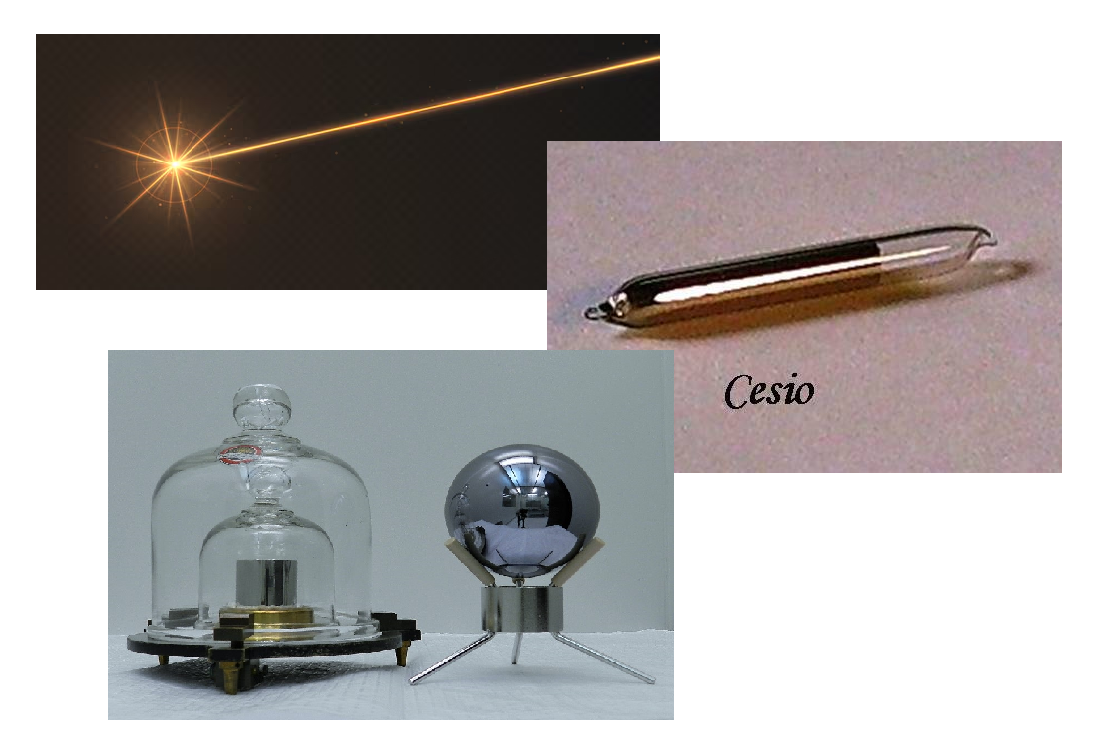
\includegraphics[width=0.8\linewidth]{figures/que-se-mide.png}
    \end{figure}

    Por ejemplo, para medir distancia, comparemos con la luz. Para medir masas, comparemos con objetos que nunca más volveremos a tocar. Para medir tiempo, comparemos con átomos.    
\end{frame}

\begin{frame}{¿Qué podemos medir?}

\textbf{Magnitud física}

    Una magnitud física es toda propiedad de un fenómeno, cuerpo o sustancia que se puede medir y expresar con un número y una unidad.
    
    \vspace{1em}

    \begin{columns}
        \column{0.45\textwidth}
        \textbf{Fundamentales}
        
        Se definen por sí mismas
        \begin{itemize}
            \item Tiempo
            \item Longitud
            \item Masa
            \item Temperatura
            \item Cantidad de sustancia
            \item Intensidad luminosa
            \item Carga eléctrica
        \end{itemize}
        $$\vdots$$
        
        \column{0.45\textwidth}
        \textbf{Derivadas}
        
        Se obtienen a partir de las fundamentales
        \begin{itemize}
            \item Velocidad
            \item Aceleración
            \item Fuerza
            \item Potencia
            \item Energía
            \item Corriente eléctrica
        \end{itemize}
        $$\vdots$$
    \end{columns}
\end{frame}

\begin{frame}{¿Qué referencias usamos para medir?}
\textbf{Unidades de medida}

Las unidades de medida son estándares o referencias que se usan para expresar el valor de una magnitud física.

\vspace{1em}

\textit{Ejemplos:} metros, pulgadas, yardas, segundos, eones, años, gramos, coulombs, newtons, amperios, voltios, celcius, parsec, años luz, candelas, etc.

\end{frame}

\begin{frame}{¿Qué estándares usamos para medir?}
    \textbf{Sistemas de medida}

Un sistema de medida es un conjunto organizado de unidades de medida y reglas que se usan para medir y expresar magnitudes físicas de forma uniforme.

Es como un “idioma común” para las mediciones: define qué unidades usar y cómo relacionarlas.

    \begin{table}[h]
\centering
\caption{Unidades base del Sistema Internacional (SI)}
\begin{tabular}{|l|l|l|}
\hline
\textbf{Magnitud} & \textbf{Unidad} & \textbf{Símbolo} \\ \hline
Longitud & metro & m \\ \hline
Masa & kilogramo & kg \\ \hline
Tiempo & segundo & s \\ \hline
Temperatura & kelvin & K \\ \hline
Corriente eléctrica & amperio & A \\ \hline
Cantidad de sustancia & mol & mol \\ \hline
Intensidad luminosa & candela & cd \\ \hline
\end{tabular}
\end{table}
\end{frame}

\begin{frame}
    \begin{table}[h]
\centering
\caption{Unidades comunes en el sistema inglés}
\begin{tabular}{|l|l|l|}
\hline
\textbf{Magnitud} & \textbf{Unidad} & \textbf{Símbolo} \\ \hline
Longitud & pie & ft \\ \hline
Longitud & pulgada & in \\ \hline
Masa & libra & lb \\ \hline
Tiempo & segundo & s \\ \hline
Temperatura & grado Fahrenheit & $^\circ$F \\ \hline
Fuerza & libra-fuerza & lbf \\ \hline
Velocidad & milla por hora & mph \\ \hline
\end{tabular}
\end{table}

\end{frame}

\begin{frame}{Equivalencias entre sistemas}
\footnotesize
    \begin{table}[h]
\centering
\caption{Equivalencias entre el Sistema Internacional y el Sistema Inglés}
\begin{tabular}{|l|l|l|}
\hline
\textbf{Magnitud} & \textbf{Sistema Internacional (SI)} & \textbf{Sistema Inglés} \\ \hline
Longitud & 1 metro (m) = 3.2808 pies (ft) & 1 pie (ft) = 0.3048 m \\ \hline
Longitud & 1 kilómetro (km) = 0.6214 millas (mi) & 1 milla (mi) = 1.6093 km \\ \hline
Masa & 1 kilogramo (kg) = 2.2046 libras (lb) & 1 libra (lb) = 0.4536 kg \\ \hline
Fuerza & 1 newton (N) = 0.2248 libras-fuerza (lbf) & 1 lbf = 4.4482 N \\ \hline
Velocidad & 1 m/s = 2.2369 millas/hora (mph) & 1 mph = 0.4470 m/s \\ \hline
Temperatura & $^\circ$C = ($^\circ$F - 32) × 5/9 & $^\circ$F = ($^\circ$C × 9/5) + 32 \\ \hline
\end{tabular}
\end{table}

\end{frame}

\begin{frame}{Ejemplos}

\textbf{Ejemplo 1: Inglés $\rightarrow$ SI}  

Convertir \SI{12}{\foot} a metros:

\[
\SI{12}{\foot} \times \frac{\SI{0.3048}{\metre}}{\SI{1}{\foot}} 
= \SI{3.6576}{\metre}
\]

\textbf{Ejemplo 2: SI $\rightarrow$ Inglés}  

Convertir \SI{5}{\metre} a pies:

\[
\SI{5}{\metre} \times \frac{\SI{3.2808}{\foot}}{\SI{1}{\metre}} 
= \SI{16.404}{\foot}
\]
\end{frame}

\begin{frame}{¿Cómo evitamos números muy largos?}

\textbf{Prefijos}

    Los prefijos son partículas que se colocan delante del nombre o símbolo de una unidad para indicar que la magnitud medida es un múltiplo o un submúltiplo de esa unidad.

En otras palabras, los prefijos nos ahorran escribir muchos ceros, tanto a la izquierda como a la derecha de la coma decimal.
\end{frame}

\begin{frame}

\footnotesize

    \begin{table}[h]
\centering
\begin{tabular}{|l|l|l|}
\hline
\textbf{Prefijo} & \textbf{Símbolo} & \textbf{Factor de multiplicación} \\ \hline
yotta  & Y  & $10^{24}$  \\ \hline
zetta  & Z  & $10^{21}$  \\ \hline
exa    & E  & $10^{18}$  \\ \hline
peta   & P  & $10^{15}$  \\ \hline
tera   & T  & $10^{12}$  \\ \hline
giga   & G  & $10^{9}$   \\ \hline
mega   & M  & $10^{6}$   \\ \hline
kilo   & k  & $10^{3}$   \\ \hline
hecto  & h  & $10^{2}$   \\ \hline
deca   & da & $10^{1}$   \\ \hline
—      & —  & $10^{0}$   \\ \hline
deci   & d  & $10^{-1}$  \\ \hline
centi  & c  & $10^{-2}$  \\ \hline
milli  & m  & $10^{-3}$  \\ \hline
micro  & $\mu$ & $10^{-6}$  \\ \hline
nano   & n  & $10^{-9}$  \\ \hline
pico   & p  & $10^{-12}$ \\ \hline
femto  & f  & $10^{-15}$ \\ \hline
atto   & a  & $10^{-18}$ \\ \hline
zepto  & z  & $10^{-21}$ \\ \hline
yocto  & y  & $10^{-24}$ \\ \hline
\end{tabular}
\end{table}
\end{frame}

\begin{frame}{Ejemplos}
    \begin{itemize}
    \item \SI{1}{\kilo\metre} $\;=\;$ 1000 metros $\;=\;$ $10^{3} \ \si{\metre}$
    \item \SI{1}{\milli\metre} $\;=\;$ 0.001 metros $\;=\;$ $10^{-3} \ \si{\metre}$
    \item \SI{1}{\micro\second} $\;=\;$ 0.000001 segundos $\;=\;$ $10^{-6} \ \si{\second}$
\end{itemize}
\end{frame}

\begin{frame}
    \begin{center}
        \Huge ¿Preguntas?
    \end{center}
\end{frame}